\section{Experiments}
\label{sec:exp}

In this section we present our instance-based POS induction
experiments.  Section~\ref{sec:evaluation} describes the accuracy
metrics that we use to evaluate our results.  Section~\ref{sec:expset}
details the test corpus and the experimental parameters used in the
English experiments and compares our results with previous work.  
%% Section~\ref{sec:instance} presents the
%% performance of our instance based model on English POS induction and
%% performs sensitivity analysis.  
Section~\ref{sec:typevsinstance}
compares the performance of type and instance based systems on
ambiguous words.  Finally, Section~\ref{sec:multilang} extends the
language and corpus coverage by applying the best performing instance
based models to 19 corpora in 15 languages.

%% Clustering results on word types, first presented in
%% \cite{yatbaz-sert-yuret:2012:EMNLP-CoNLL}, are still state of the art for
%% English POS induction.  However in this study we show that the performance on
%% ambiguous words can be further improved by clustering word instances. 
%% (Sections~\ref{sec:clustering-s} and \ref{sec:clustering-c}), we improve the
%% model that incorporates morphological and orthographic features
%% (Section~\ref{sec:feat} and Appendix~C), and we demonstrate the applicability
%% of our methods to other languages (Section~\ref{sec:multilang}).
\subsection{Evaluation}
\label{sec:evaluation}
We report many-to-one and V-measure scores for our experiments as
suggested in \cite{Christodoulopoulos:2010:TDU:1870658.1870714}.  The
many-to-one (\mto) evaluation maps each cluster to its most frequent
gold tag and reports the percentage of correctly tagged instances.
The \mto\ score can be increased by simply increasing number of
clusters, thus the number of clusters is fixed to match the number of
gold tags in each experiment.  The V-measure (\vm)
\cite{rosenberg2007v} is an information theory motivated metric that
calculates the harmonic mean of completeness and homogeneity of the
clusters.  Completeness of a cluster is maximized when all instances
of a gold-tag are grouped into the same cluster and the homogeneity is
maximized when the members of a cluster belong to the same gold-tag.
%% In Section~\ref{sec:discuss} we argue that
%% homogeneity is perhaps more important in part of speech induction and
%% suggest \mto\ with a fixed number of clusters as a more intuitive
%% metric.

\subsection{Experimental Settings and Results}
\label{sec:expset}

To make a direct comparison with previously published results,
% what is the test data
the Wall Street Journal Section of the Penn Treebank was used as the
test corpus (1,173,766 instances, 49,206 unique tokens) for English
experiments.
% what is the tag set
PTB uses 45 part-of-speech tags which we used as the gold standard for
evaluation in our experiments.

% what is the LM training data
%Train => 88214605 2303225131 12630027619
To compute substitutes in a given context we trained a language model
using the ukWaC corpus ($\approx$ 2 billion tokens) constructed by
crawling the ``.uk'' Internet
domain \cite{ferraresi2008introducing}\footnote{We use the Penn
  Treebank Tokenizer to make the training data compatible with PTB.}.
% how is the language model trained
We used SRILM \cite{Stolcke2002} to build a 4-gram language model with
interpolated Kneser-Ney discounting.
% what is the vocabulary
Words that were observed less than 2 times in the language model
training data were replaced by \unk\ tags, which gave us a
vocabulary size of 4,254,946. 
% what is the test data
% perplexity
The perplexity of the 4-gram language model on the PTB is 303 and the
unknown word rate is 0.008.  For computational efficiency only the top
100 substitutes and their probabilities were computed for each
position in the PTB using the {\sc fastsubs} algorithm \cite{yuret2012fastsub}.  
% (1,173,766 instances, 49,206 types)
%% The probability vectors for each position were normalized to add up to
%% 1.0 giving us the final substitute distributions used in our
%% experiments.
We use the same orthographic features defined in
\cite{yatbaz-sert-yuret:2012:EMNLP-CoNLL} and generated morphological
features using the unsupervised algorithm Morfessor \cite{creutz05}.
%% Morfessor was trained on PTB using default settings, and a perplexity
%% threshold of 300.  We concern only the splits tagged as {\em suffix}
%% in the Morfessor output and allow at most one morphological feature
%% per word type \footnote{Splits are concatenated if there are
%%   consecutive suffix parts at the end of a word type.}.

%TODO: define phi_0, nu_0 in appendix.
% To make a meaningful comparison on the PTB
The experiments were run using the following default settings (unless otherwise
stated): (1) each word was kept with its original capitalization; (2) 90
substitutes sampled per instance; (3) the learning rate parameters for S-CODE
were set to $\varphi_0=50$, $\eta_0=0.2$; (4) S-CODE convergence threshold,
the log-likelihood difference between two consecutive iterations, was set to
0.001; (5) the S-CODE dimensions and $\tilde{Z}$ were set to 25 and 0.166,
respectively; (6) a modified k-means algorithm with smart initialization was
used \cite{arthur2007k}; (7) the number of k-means restarts was set to
128 to improve clustering and reduce variance.

Each experiment was repeated 10 times with different random seeds and
the results are reported with standard errors in parentheses or error
bars in graphs.  Table~\ref{tab:results} summarizes all the results
reported in this section and the ones we cite from the literature.

%\FloatBarrier
\begin{table}[t] 
\centering  \small
%\begin{tabular}{|@{ }l@{ }|@{ }l@{ }|@{ }l@{ }|}
%%\hline
%%Distributional Models & \mto & \vm \\
%%\hline
%%Lamar et al. \shortcite{Lamar:2010:LCU:1870658.1870736} & .708 & -\\ %algorithm name LDC
%%Brown et al. \shortcite{Brown:1992:CNG:176313.176316}* & .678 & .630\\
%%%kcls(Och,1999) & .737 & .656\\
%%%\cite{goldwater-griffiths:2007:ACLMain} & .632 & .562\\
%%Goldwater et al. \shortcite{goldwater-griffiths:2007:ACLMain}* & .632 & .562\\
%%Ganchev et al. \shortcite{Ganchev:2010:PRS:1859890.1859918}* & .625 & .548\\
%%Maron et al. \shortcite{maron2010sphere} & .688 (.0016)&-\\
%%{\bf Substitutes(instances)} (Sec.~\ref{sec:instance}) & \wsxymto & \wsxyvm \\
%%Yatbaz et al. \shortcite{yatbaz-sert-yuret:2012:EMNLP-CoNLL} & .7680 & .6822 \\
%%\hline
%%\end{tabular}
%\begin{tabular}{|@{ }l@{ }|@{ }l@{ }|@{ }l@{ }|}
  \begin{tabular}{|l|l|l|}
\hline
Model & \mto & \vm \\
\hline
Clark \shortcite{Clark:2003:CDM:1067807.1067817} & .712 & .655 \\
Christodoulopoulos et al. \shortcite{christodoulopoulos-goldwater-steedman:2011:EMNLP} & .728 & .661\\
Berg-Kirkpatrick et al. \shortcite{bergkirkpatrick-klein:2010:ACL} & .755 & -\\ % Interesting in  christo paper:73.9/67.7
Christodoulopoulos et al. \shortcite{Christodoulopoulos:2010:TDU:1870658.1870714} & .761 & .688\\
Blunsom and Cohn \shortcite{blunsom-cohn:2011:ACL-HLT2011} & .775 & .697\\
Yatbaz et al. \shortcite{yatbaz-sert-yuret:2012:EMNLP-CoNLL} & .8023 (.0070) & .7207 (.0041)\\
Instance based (Sec.~\ref{sec:algorithm}) & \fwsxymto & \fwsxyvm \\
\hline
\end{tabular}
\caption{Summary of results with \mto\ and \vm\ scores.  Standard
  errors are given in parentheses when available.  All the
  models incorporate orthographic and morphological features.
  Berg-Kirkpatrick et al. \shortcite{bergkirkpatrick-klein:2010:ACL}
  and Christodoulopoulos et
  al. \shortcite{Christodoulopoulos:2010:TDU:1870658.1870714} use
  instance based models.}
\label{tab:results}
\end{table}

%% \subsection{Instance Based POS Induction} 
%% \label{sec:instance}

%% \begin{figure}[ht!] \centering
%% %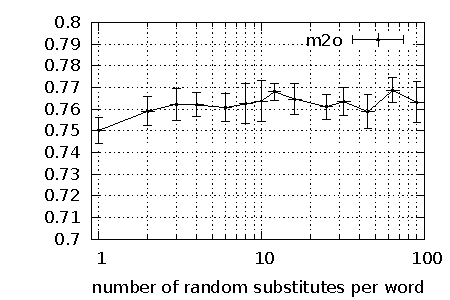
\includegraphics[width=0.5\linewidth]{plot-s.pdf}
%% 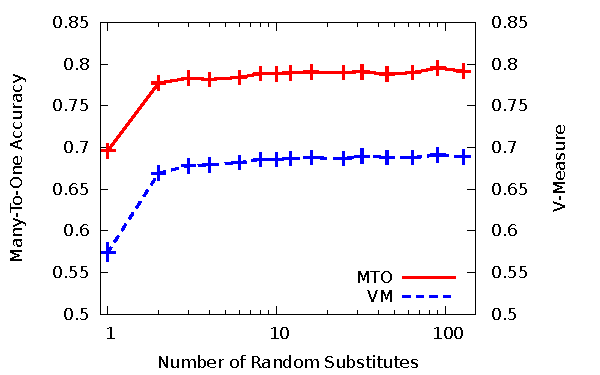
\includegraphics[width=.90\columnwidth]{plot-s-ins.pdf}
%% 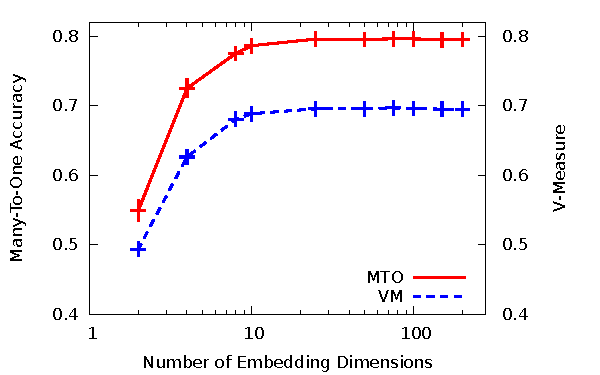
\includegraphics[width=0.90\columnwidth]{plot-d-ins.pdf}
%% 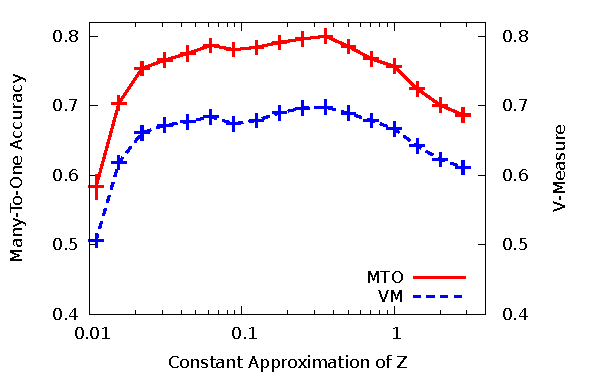
\includegraphics[width=0.90\columnwidth]{plot-z-ins.pdf}
%% %% \caption{\mto\ and \vm\ are not sensitive to the number of random substitutes
%% %% sampled per word instance.}
%% \caption{Sensitivity of instance-based POS induction performance on
%%   the PTB to (a) the number of sampled substitutes, (b) the number of
%%   embedding dimensions, (c) the constant approximation to the
%%   normalization constant $\tilde{Z}$.
%% }
%% \label{plot-s}
%% \end{figure}

%% % TODO: This goes to algorithm section:
%% %% S-CODE uses stochastic gradient ascent to find the $\phi_w, \psi_c$ embeddings
%% %% for words types and contextual features on a 25-dimensional unit sphere.  The algorithm
%% %% cycles through the word-features tuple data until it converges.  
%% We construct a vector representation for instances by concatenating the S-CODE
%% embedding of the target word $\phi_w$ with the average of sampled substitute
%% embeddings, $\overline{\psi_c}$.  The resulting $\phi_w \oplus
%% \overline{\psi_c}$ vectors are clustered using the k-means algorithm and the
%% cluster-id for each $\phi_w \oplus \overline{\psi_c}$ becomes the predicted
%% category of the corresponding word instance.  Using the default settings the
%% many-to-one accuracy on the PTB is \fwsxymto\ and the V-measure is \fwsxyvm.
%% %% Moved to appendix
%% %% To obtain a discrete representation of the context, the
%% %% random-substitutes algorithm pairs each word instance with a substitute
%% %% sampled from the pre-computed substitute vectors generated from the
%% %% word instance's context (see Section~\ref{sec:subcomp}) and word ($X$) --
%% %% random-substitute ($Y$) pairs are fed to the S-CODE as input.  It is
%% %% possible (and beneficial, see below) to run the random-substitutes
%% %% algorithm on the data more than once to generate more pairs from the
%% %% same substitute vectors. 
%% %% To obtain a discrete representation of the context, the
%% %% random--partitions algorithm first designates a random subset of
%% %% substitute vectors as centroids to partition the space, and then
%% %% associates each context with the partition defined by the closest
%% %% centroid in cosine distance.  Each partition thus defined gets a
%% %% unique id, and word ($X$) -- partition-id ($Y$) pairs are given to
%% %% S-CODE as input.  The algorithm uses stochastic gradient ascent to
%% %% find the $\phi_x, \psi_y$ embeddings for word and partition-id in
%% %% these pairs on a single 25-dimensional sphere.  The algorithm cycles
%% %% through the data until we get approximately 50 million updates.  The
%% %% resulting $\phi_x$ vectors are clustered using an instance weighted
%% %% k-means algorithm and the resulting groups are compared to the correct
%% %% part of speech tags.  Using default settings with 64K random
%% %% partitions the many-to-one accuracy is \rpmto\ and the V-measure is
%% %% \rpvm.
%% % \subsubsection*{Sensitivity Analysis}

%% To analyze the sensitivity of this result to our specific parameter
%% settings we ran a number of experiments where each parameter was
%% varied over a range of values.
%% %% \begin{figure}[ht] \centering
%% %% 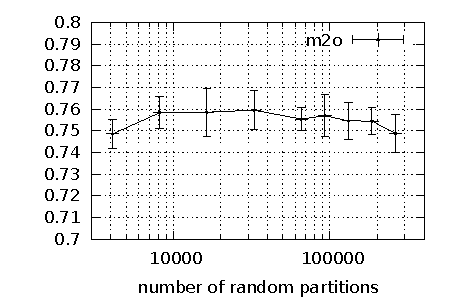
\includegraphics[width=0.5\linewidth]{plot-p.pdf}
%% %% \caption{\mto\ is not sensitive to the number of partitions used to
%% %%   discretize the substitute vector space within our experimental
%% %%   range.}
%% %% \label{plot-p}
%% %% \end{figure}
%% %% Figure~\ref{plot-p} gives results where the number of initial random
%% %% partitions is varied over a large range and shows the results to be
%% %% fairly stable across two orders of magnitude.

%% The first plot in Figure~\ref{plot-s} illustrates that the result is
%% fairly robust with respect to the number of random substitutes sampled
%% for each target word instance, as long as the training algorithm can
%% observe more than a few random substitutes per word.  The second plot
%% shows that at least 10 embedding dimensions are necessary to get
%% within 1\% of the best result, but there is no significant gain from
%% using more than 25 dimensions.  The third plot shows that the constant
%% $\tilde{Z}$ approximation can be varied within two orders of magnitude
%% without a significant performance drop in the scores.  For uniformly
%% distributed points on a 25 dimensional sphere, the expected $Z$ is
%% $0.146$.  In the experiments where we tested we found the real $Z$
%% always to be in the 0.140-0.170 range.  When the constant $\tilde{Z}$
%% estimate is too small, all points tend to converge to the same
%% location.  When $\tilde{Z}$ is too high, it prevents meaningful
%% clusters from coalescing.

